\section{Rešavani problem}

\subsection{Opis problema}

\textit{5.25" flopi disketa} je istoriski primerak medijuma koji je korišćen za  \newline skladištenje podataka. Razvojem računarstva i postizanjem boljih performansi računara kao i potrebama za većom količinom memorije ovaj medium je izgubio svoje mesto na tržištu i preselio se u istoriju. Njegove karakteristike nisu mogle da ispune ni prostorne a ni performansne potrebe.  Vreme je pregazilo ovaj medium a da bi se sačuvali podaci i zabeležio bitan deo istorije pribegavano je skaldištenju i čuvanju podataka u \textit{D64 fajlovima}.

Prilikom čitanja \textit{5.25"flopi diskete} i prebacivanja njenih podataka u elektronski oblik odnosno \textit{D64 fajl} dolazi do pojave grešaka na nekim sektorima. Nastale greške prilikom čitanja se skladište u dodatnim bajtovima na kraju \textit{D64 fajla} i dalja evidencija grešaka se vrši isključivo preko ovih dodatnih bajtova. Ovaj problem je predstavljao kamen spoticanja prilikom arhiviranja podataka sa ovih mediuma. Kao uzrok možemo navesti zastarelost tehnologije, kao i oštećenost mediuma. Primer jednog lošeg čitanja prikazan je na slici \ref{img:loseCitanje} gde crvena boja označava sektore sa greškom a zelena ispravne.

\begin{figure}[ht]
\begin{center}
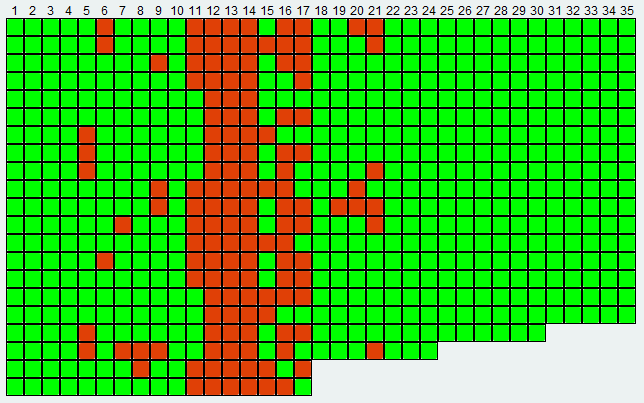
\includegraphics{img/loseCitanje.png}
\caption{Loše čitanje 5.25" flopi diskete}
\label{img:loseCitanje}
\end{center}
\end{figure}

\subsection{Analiza problema}

Kao što je već rečeno prilikom čitanja \textit{5.25" flopi disketa} dolazi do  \newline neželjenih grešaka nad pojedinim sektorima, odnosno određeni sektori nisu dobro pročitani. Zbog analize ovog problema realizovano je programsko rešenje koje na osnovu dodatnih bajtova na kraju \textit{D64 fajla} omogućuje vizuelnu predstavu sekotra. Ispravni sektori obeleženi su zelenom bojom dok su neispravni obeleženi crvenom o softveru više u nastavku. Analizom  \textit{D64 fajlova} ustanovljeno je da se prilikom višestrukog čitanja iste flopi diskete javljaju greške u različitim sektorima, odnosno da prilikom prvog i drugog čitanja nisu isti sektori pogrešno pročitani. Vizuelni prikaz dva  \textit{D64 fajla}  iste \textit{5.25" flopi diskete} prikazan je na slici \ref{img:visestrukoCitanje}.

\begin{figure}[ht]
\begin{center}
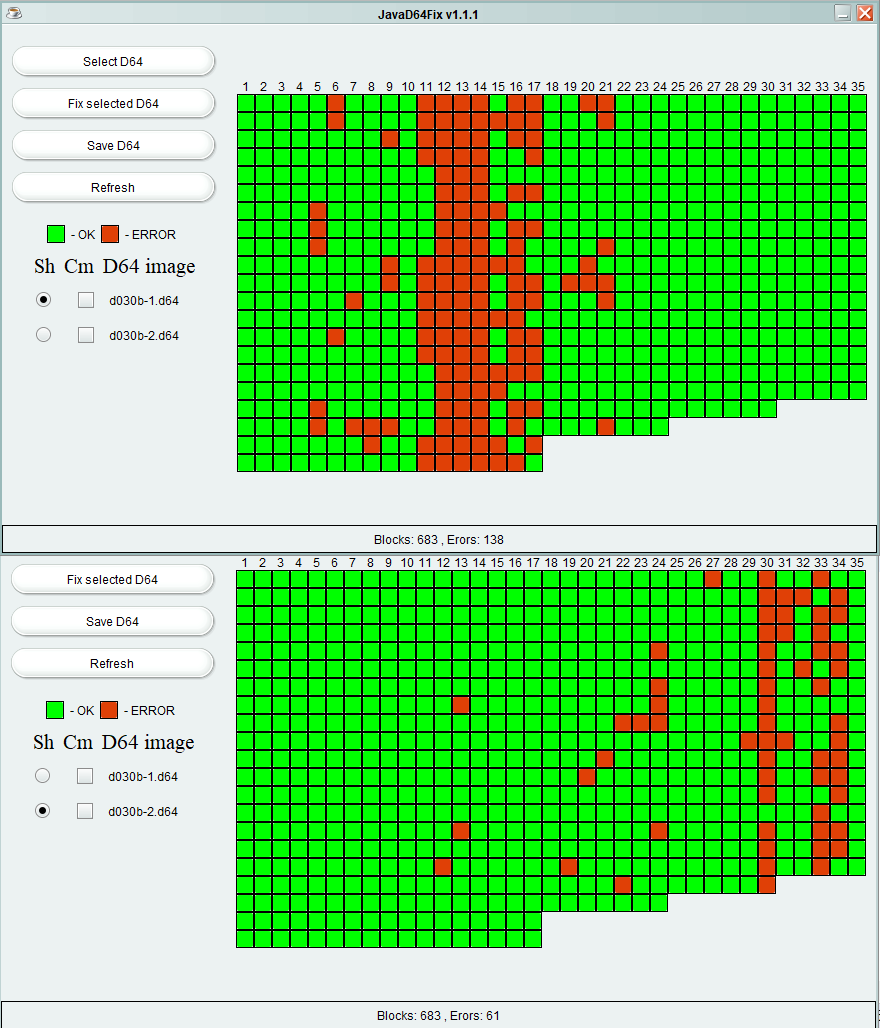
\includegraphics[width=11cm]{img/visestrukoCitanje.png}
\caption{Višestruko čitanje iste 5.25" flopi diskete}
\label{img:visestrukoCitanje}
\end{center}
\end{figure}